%!TEX root =../../thesis-ex.tex

\chapter{Recommending Explanation to Assist Security Decision Making}
\label{ch4:clap}

Security and privacy on mobile devices has been a challenging task~\cite{journals/tocs/EnckGHTCCJMS14,conf/ccs/FeltCHSW11,conf/soups/FeltHEHCW12,conf/huc/LinSALHZ12,conf/soups/LinLSH14,yang2015appcontext}. Recently user privacy gathered new attentions following the Facebook-Cambridge Analytica data scandal~\cite{facebookleak}. The current solution for user privacy protection on the Android platform mainly relies on a permission mechanism, i.e., apps have to request permissions before getting access to sensitive resources. 
Unfortunately, previous work~\cite{conf/ccs/FeltCHSW11} finds that apps frequently request more permissions than the apps need. 
To reduce users' concerns toward those \emph{over-privileged apps}~\cite{conf/ccs/FeltCHSW11,journals/tocs/EnckGHTCCJMS14} and improve the users' understanding of permission usages~\cite{conf/soups/ChinFSW12,conf/chi/KelleyCS13}, one effective approach is to give the users warnings by showing natural language explanations~\cite{conf/huc/LinSALHZ12}. 
For instance, WHYPER~\cite{conf/uss/PanditaXYEX13} uses app description sentences to explain permissions; Android and iOS also launched their features of runtime permission explanations in 2015 and 2012, respectively. 

\begin{figure}[t]
\centering
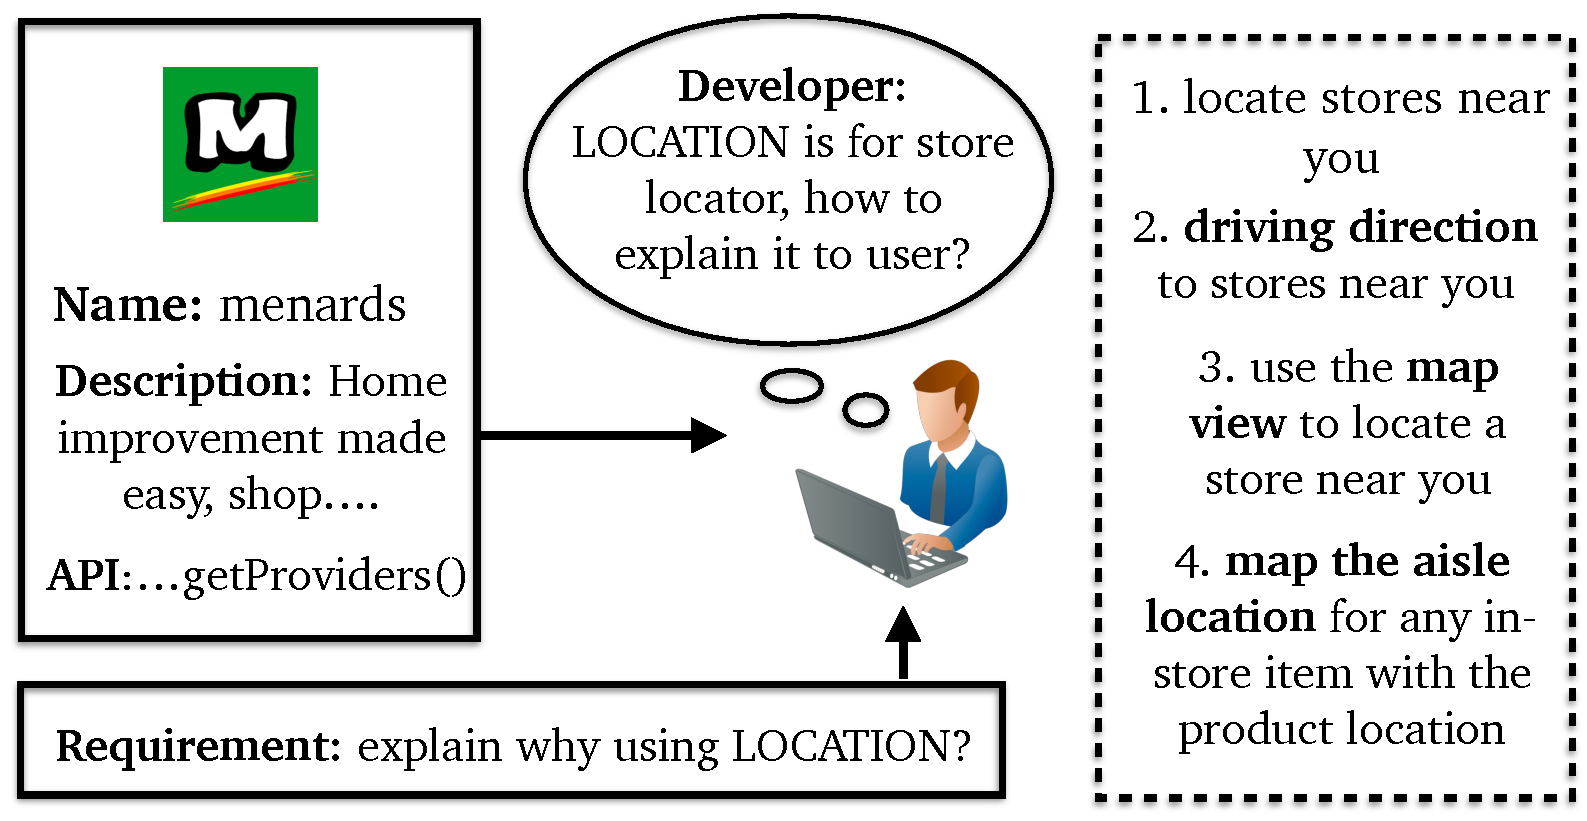
\includegraphics[width=0.45\textwidth]{figure/chapter2/intro-crop.pdf}
\caption{An example showing how CLAP assists developers with permission requirements, with the dashed rectangle showing sentences recommended by CLAP.}
\label{fig:intro}
\vspace{-0.2in}
\end{figure}

% describe three challenges in writing a good explanation sentence
Permission explanations are short sentences that state the purpose of using a permission. 
Permission explanations are written by Android developers~\cite{conf/chi/TanNTNTEW14}; 
within our knowledge, there exists no previous work on studying the steps of multi-stakeholder elicitation~\cite{requirementelicitation} or requirements  specification~\cite{requirementspecification} for writing such sentences. Without these steps, can we rely solely on developers' decisions to explain permissions? 
Although there exist many good examples of app explanations, it is unclear whether explanations provided by developers are interpretable from an average user's perspective. 
In particular, three major challenges can reduce the interpretability of an explanation sentence. 
(1) \emph{Technical Jargons}. Due to the domain knowledge owned by the developers but not the average users, the developers' explanations sometimes contain technical jargons/logics hard for the average users to understand. 
For example, app \emph{GeoTimer Lite} explains the location permission as for ``\emph{geofence}''~\cite{geolite}; however, the average users may not know the meaning of geofence, not to say why geofence requires the location permission~\cite{geofence}. 
(2) \emph{Optimal Length}. If the explanation is too short, it is likely ambiguous (e.g., in Figure~\ref{fig:intro}, it is unclear whether ``\emph{store locator}'' refers to a locator outside or inside the store); 
on the other hand, if the explanation is long and wordy, users may choose to skip it. 
It can be challenging for the developers alone to make the decision on the length/degree of detailedness.
(3) \emph{Rare Permission Usage}. Although it is relatively easy to explain commonly acknowledged permission usages, e.g., the location permission in a GPS app, it becomes much more challenging to \emph{clearly} explain rare permission usages. 

After identifying difficulties in explaining permissions, we propose the first study on the requirements specification/discovery of permission explanations, and we call it the process of \emph{permission requirements discovery}. 
In particular, we build a recommender system, which recommends a list of potential requirements for the permission explanation (i.e., sentences from similar apps' descriptions\footnote{Alternatively, we can also use privacy documents and runtime permission messages. However, both data sources are much more scarce than app descriptions. As a result, we choose to use app descriptions.
However, the two data resources are both applicable to the CLAP framework.}) so that developers could refer to the list for improving the interpretability of their explanations. 
In Figure~\ref{fig:intro}, we illustrate how our system helps the developer of an app discover the requirements. 
First, by observing sentence 2 and sentence 4, the developer finds the current explanation ``\emph{store locator}'' ambiguous, and then explicitly specifies indoor/outdoor; 
second, by observing the keyword ``\emph{map}'' in sentence 3, the developer is reminded of the map feature and adds it to the explanation; 
finally, by observing sentence 4, the developer discovers a new feature, i.e., indoor locator, to be added to the app. 

Because our recommender system leverages similar apps' descriptions, we name it CLAP, which is the abbreviation for $\underline{\textbf{C}}$o$\underline{\textbf{L}}$laborative $\underline{\textbf{A}}$pp $\underline{\textbf{P}}$ermission recommendation. 
CLAP uses the following four-step process to recommend a list of candidate sentences. 
First, based on information from the current app (the current app's title, description, permissions, or category), CLAP leverages a text retrieval technique to rank every app from the dataset (Section~\ref{sec:similar}). 
Second, for every top-ranked app, CLAP goes through every sentence in its description text and assesses whether the sentence explains the target permission (Section~\ref{sec:keywords}). 
CLAP further processes matched sentences so that each sentence contains only one explanation (Section~\ref{sec:candidate}). Third, CLAP aggregates text information of the top-K similar apps, and uses the aggregated word values to re-rank the candidate sentences found in the previous step (Section~\ref{sec:vote}). 
Finally, for top re-ranked sentences, CLAP post-processes the sentences to remove duplications and to improve their interpretability (Section~\ref{sec:postprocess}). 

% evaluation
We evaluate CLAP's performance (Section~\ref{sec:exp}) on a large dataset consisting of 1.4 million Android apps. 
First, we examine the relevance of recommended sentences. \tabularnewline
To evaluate the relevance, we extract the purpose-explaining sentences from 916 apps as the gold standard sentences, and compare CLAP-recommended sentences with the gold-standard sentences. 
The evaluation results show that CLAP has a high relevance score compared with existing state-of-the-art approaches~\cite{conf/uss/PanditaXYEX13}. 
Second, we conduct a qualitative study on specific examples, to observe to what extent the CLAP results can help with the interpretability. 
The study results show that CLAP can effectively recommend candidate sentences that are concise, convey specific purposes, and support a diverse choice of re-phrasing for the same purpose. 
These characteristics show great promise of CLAP in helping developers find more interpretable explanations and bridging the knowledge gap between different stakeholders' viewpoints. 


This paper makes the following three main contributions: 
%{\bf Cheng: we need to make at least one contribution relevant to requirements engineering}
\begin{itemize}
  \item We make the first attempt to study the problem of permission requirements discovery, with a focus on  %{\color{red}{
  explaining an app's permission to users. 
%}}
  %especially when such explanation is not found in the description of the app itself.
  % for app developers to explain an app's permission
  \item We propose a novel CLAP framework for addressing the formulated problem by leveraging similar apps' permission-explaining sentences.
  \item We evaluate CLAP on a large dataset and show that CLAP effectively provides highly relevant explaining sentences, showing great promise of CLAP as an assistant for requirements discovery of app-permission explanations. 
\end{itemize}

% The rest of this paper is organized as follows. Section~\ref{sec:tradeoff} motivates the CLAP framework. Sections~\ref{sec:identify} -~\ref{sec:postprocess} introduce the four-step process of the CLAP framework: identifying explaining sentences  (Section~\ref{sec:identify}),  finding similar apps (Section~\ref{sec:similar}),  voting explaining sentences (Section~\ref{sec:vote}), and post-processing resulting sentences (Section~\ref{sec:postprocess}). Section~\ref{sec:exp} presents the evaluation results on three  security-sensitive permissions. Section~\ref{sec:relwork} discusses related work. Finally, Section~\ref{sec:conclusion} discusses future work, limitations of CLAP, and concludes the paper.

%!TEX root =../main.tex

% Life's more fun when you live in the moment :) Happy Snapping!

\section{Similar-App Ranker}
\label{sec:similar}

For the first step of the CLAP framework, we design a similar-app ranker to find apps (which also use the target permission) that are the most similar to the current app. 

We define the similarity score between the current app $Q$ and candidate app $D$ on the permission $P$ as the linear interpolation of scores in four components, 
i.e., the pairwise similarities between $Q$ and $D$'s descriptions, titles, permissions, and categories:

\vspace{-0.2in}
\begin{eqnarray}
sim(Q, D, P) &=& (\lambda_1 sim_{desc}(Q, D) \nonumber\\
&& +\lambda_2 sim_{title}(Q, D) + \lambda_3 sim_{perm}(Q, D)\nonumber\\
&& +\lambda_4 sim_{cate}(Q, D))\label{eq:simty}
\end{eqnarray}

where the coefficients $\lambda_i$'s control the importance of each component. 
Next, we describe the definitions of each similarity component. 

\subsection{Description Similarity}

To model the similarity between two descriptions, we use Okapi BM25~\cite{FT006}, In contrast, previous work~\cite{conf/icse/GorlaTGZ14} uses the topic modeling technique to capture the similarity between app descriptions. 
The reason why we choose to use a retrieval model for app descriptions is that app descriptions are usually longer texts (on average an app description contains 135 words). 
For long texts, the topic modeling technique would bring two apps together even if they only remotely belong to the same topic (instead of closely related, e.g., email apps and SMS apps are ``similar'' by the topic modeling technique, although they clearly have different functionalities). 
On the other hand, text retrieval models capture more discriminativeness between the descriptions, so they are more suitable for our problem. 

To model the text similarity using BM25, we further capture both the unigrams and bigrams from the description text. 
We stem the description texts before turning them into unigrams and bigrams. \tabularnewline
In addition to stemming, we also carry out the following pre-processing steps, which are standard pre-processing techniques in text retrieval tasks. 
These standard techniques improve the ranking performance by enhancing the discriminativeness of each app description. 

\textbf{Stop-word Removal}. We remove regular English stop words from Python's nltk stop words list~\cite{nltk}, e.g. ``\emph{the}'' and ``\emph{a}.''
Meanwhile, words such as ``\emph{Android},'' ``\emph{application},'' and ``\emph{version}'' should also be treated as stop words, because they can appear in any app. 
We identify a complete list of 294 words. 
We create the list by empirically scanning through the top frequent words, and then manually annotating whether each word can appear in any app, regardless of the context. 
The list can be found on  our project website~\cite{clapproj}.

\textbf{Background-sentence Removal}. A mobile-app description usually contains some sentences that explain common issues, e.g., ``\emph{fixed bug in version 1.7}.'' 
Same as stop words, such sentences are ``stop sentences'', which do not help explain the unique functionality of the app. 
As a result, we implement a remover of common background sentences for mobile apps using 53 regular expressions. 
Same as the creation of stop words, the creation of regular expressions is based on the empirical judgment on whether a sentence can appear in any app, e.g., \code{.*version$\backslash$s$+\backslash$d.*} detects whether a sentence describes a version number. 
The list of regular expressions can be found on our project website~\cite{clapproj}.

After the preceding pre-processing steps, we obtain the BM25 scores between the current app $Q$ and every candidate app $D$ in the dataset. 
To make the description similarity comparable to other similarity components, we normalize the BM25 scores with the maximum BM25 score over all the candidates before plugging the normalized score into Equation~\ref{eq:simty}. 

\subsection{Title Similarity}
\label{sec:titlesim}

An app's description usually offers the most information to capture its similarities with other apps~\cite{conf/icse/GorlaTGZ14}, but if CLAP uses only the descriptions, sometimes it is difficult to retrieve accurate results, due to the noisy components in descriptions that are not fully cleaned in pre-processing\footnote{For example, many app descriptions contain SEO words, which may not be strictly relevant to app functionality.}. 
To this end, app titles can serve as a complement to descriptions in modeling app similarities. 

One challenge in modeling the title similarity is the vocabulary gap between similar words, e.g., ``\emph{alarm}'' and ``\emph{wake up clock},'' mainly because titles are short texts (on average a title contains 2.8 words). 
As a result, we use a different technique to model the title similarity. 
We leverage word embedding vectors~\cite{conf/nips/MikolovSCCD13} (GoogleNews-neg300~\cite{word2vec}) for bridging the vocabulary gap. 
For each pair of apps $Q$ and $D$, we define their title similarity as the average cosine similarity between each word $w_1\in Q$ and each word $w_2\in D$. 
To avoid over-matching unrelated word pairs, we empirically cut the cosine similarities at 0.4 and set them to 0 if their original scores are less than 0.4. 

\subsection{Permission Similarity}

Because app permissions are categorical data, we model the permission similarity as the Jaccard distance between the two permission lists. 
The reason why we incorporate the permission similarity is based on the observation that an app's permissions can reflect its functionality. 
For example, emergency contact apps usually use \correcttexttt{READ\_CONTACTS} and \correcttexttt{ACCESS\_FINE\_LOCATION} at the same time, and the usage of location permission distinguishes these apps from other contact apps. 

Previous work~\cite{conf/icse/GorlaTGZ14} leverages security-sensitive APIs to model the similarity between apps. Security-sensitive APIs are a finer-grained version of Android permissions. 
Although APIs carry more information than the permissions, it is also more challenging to model the API similarity. 
The challenge comes from the fact that developers often use different APIs to achieve the same functionality (e.g., a Stack Overflow post~\cite{getcurrentlocation} shows several different techniques to obtain user location), and use the same API to achieve different functionalities.
As a result, we model only the permission-level similarity and leave the exploration of API similarity for future work. 

\subsection{Category Similarity}

Finally, we capture the category similarity between the two apps. 
The reason for using the category information is that we observe multiple cases where using only the descriptions is ambiguous.
In some cases, the category information can help clarify the apps' functionalities. 
For example, we find two apps whose descriptions are close to each other, and yet one app is a cooking app for cookie recipe while the other app is a business app for selling cookies. 
We represent each category as a TF-IDF vector, which comes from words that appear in the descriptions of apps in the category. 
The similarity between $Q$ and $D$ is defined as the cosine similarity between the two vectors.

\section{Identifying Permission-Explaining Sentences}
\label{sec:identify}

After retrieving similar apps of the current app $Q$, the next step of CLAP is to identify permission-explaining sentences among those similar apps' descriptions. 

Previous work such as WHYPER~\cite{conf/uss/PanditaXYEX13} addresses this problem (of identifying permission-explaining sentences) by matching sentences from the app description against frequent words in the permission's API documents. 
WHYPER uses only the \emph{entire} description sentences to explain the permission. 
In our problem, however, using the entire sentences can be ineffective. 
The reason for such ineffectiveness is that we are using \emph{other} apps' sentences to explain the current app. 
An entire sentence from another app sometimes contains redundant information: while a part of the sentence matches the current app's purpose, the other part does not match it. 
For example, the sentence ``\emph{save the recording as a ringtone and share it with your friends}'' describes the usages of two permissions: \correcttexttt{RECORD\_AUDIO} and \correcttexttt{READ\_CONTACTS}, whereas the current app uses only the first permission. 
If we use the entire sentence to explain the current app, the second part is irrelevant, whereas if we discard the entire sentence, the relevant part is also discarded. 
In such cases, if we break the original sentence into shorter units, the first part will contain only the relevant information. 
CLAP leverages this methodology to break the original sentence into shorter ones so that some of them are more relevant than the original sentence. 
We describe this process in Section~\ref{sec:candidate}. 

\subsection{Breaking Sentences into Individual Purposes}
\label{sec:candidate}

% recursively traverse the parsing tree and split a phrase if it contains at least one conjunction.

To break a sentence into shorter ones, we leverage the Stanford PCFG parser~\cite{Klein2003} to parse each sentence $s$ into a tree $T$. 
In particular, we extract its sub-sentences based on two main observations. 
First, following the aforementioned example, if the sentence contains conjunction(s), we split it at the conjunction(s), and then extract the sub-sentences. 
Second, as discussed in previous work~\cite{conf/uss/PanditaXYEX13,conf/ccs/QuRZCZC14}, permission usages can usually be captured by short verb phrases, e.g., ``\emph{create QR code from contact},'' ``\emph{assign contact ringtone}.'' 
Therefore, we also extract the verb phrases in the sentence. 

After the split, CLAP adds both the original sentence and the shorter sentences into a candidate sentence set, which is then passed on to the next step for identifying permission-explaining sentences. 
We intend to include as many candidate sentences as possible to boost the quality of the finally chosen ones. 
Therefore, when we traverse the parsing tree $T$, we keep all the verb phrases; e.g., if one verb phrase is embedded in another, we include both of them in the candidate set. 

We summarize our candidate-sentence generator in Algorithm~\ref{algo} for a clearer view, where $s(n)$ denotes the phrase (in sentence $s$) corresponding to node $n$. 

\begin{algorithm}
\caption{Constructing Candidate Set\label{algo}}
\DontPrintSemicolon
  \SetKwInOut{Input}{Input}
  \SetKwInOut{Output}{Output}
  \Input{Sentence $s$ and its tree structure $T$ obtained from constituent parsing~\cite{Klein2003};}
  \Output{Candidate sentences $S$ from $s$;}
  $S\leftarrow\emptyset;$\;
  $S\leftarrow S \cup \{s\}$;\tcp*{add the original sentence}
  \For{node $n$ in T}{
   \If{$n = VP$}{
   		$S\leftarrow S\cup \{s(n)\}$;\tcp*{add verb phrase}
   }
    \If{$n = CC$}{
  		\For{node $n_0$ in $n.parent.children$ and $n_0 != CC$}{
  			$S\leftarrow S\cup \{s(n_0)\}$;\tcp*{break  conjuncts}
  		}
  		}
  }
\end{algorithm}
\vspace{-0.2in}

\subsection{Matching Permission-Explaining Sentences}
\label{sec:keywords}

\textbf{Using Keyword Matching}. After obtaining the candidate sentence set from the preceding step, we use a pre-defined set of rules to match each candidate sentence, and keep only those sentences that address the target permission. 
More specifically, the pre-defined set of rules include keywords and POS tags~\cite{conf/naacl/ToutanovaKMS03}. 
The reason why we leverage the POS tags is to disambiguate between a word's senses based on its tag. 
For example, when the word ``\emph{contact}'' is used as a noun, it usually refers to phone contacts, so it explains \correcttexttt{READ\_CONTACTS}, whereas if it is used as a verb, e.g., ``\emph{contact us through email},'' it does not explain \correcttexttt{READ\_CONTACTS}. 
The pre-defined keywords and POS tags set can be found on our project website~\cite{clapproj}. 

\textbf{Using WHYPER to Match Sentences}. Alternatively, we can use WHYPER in this step. 
The reason why we use the keyword matching is for a low time cost and for real-time processing. 
WHYPER traverses the entire dependency parsing graph. 
This step makes WHYPER run at least 100 times slower than the keyword matching. 
Meanwhile, the size of our data dictates that we need to process tens of millions of sentences for each permission. 
As a result, we use keyword matching to speed up this step. We plan to support WHYPER in future extensions of CLAP.

After the preceding steps, we discard apps that CLAP has not identified any sentences from. 

%!TEX root =../main.tex
\section{Ranking Candidate Explaining Sentences}
\label{sec:vote}

After the preceding steps, CLAP obtains similar apps and candidate permission-explaining sentences. 
Next, CLAP ranks the candidate sentences and recommends the top sentences to the developer. 

\textbf{Why Ranking Sentences?} After obtaining explaining sentences, a straightforward technique for recommending sentences is the greedy technique, i.e., scanning through the app list top-down and extracting the first 5 sentences. 
However, this simple technique makes mistakes for the following two reasons.  
First, due to the noise in the data, the retrieved similar apps inevitably contain false positive ones\footnote{After exploring three retrieval techniques: BM25~\cite{FT006}, language model~\cite{Zhai07noteson}, and vector space model~\cite{361220}, we find that all the techniques generate false positive results. 
Such results are due to noisy components in the app descriptions, e.g., SEO words that are sometimes irrelevant to the primary app functionality. }. 
As a result, it is very likely for the greedy technique to select sentences from a mismatched app; sentences from mismatched apps usually discuss different purposes. 
Second, even if an app is correctly matched, it may still use the same permission for a different purpose. 
For example, an alarm app may use \correcttexttt{ACCESS\_FINE\_LOCATION} for weather report and advertisement at the same time. 

\textbf{Ranking Candidate Sentences with Majority-Voting. } Because the greedy technique could easily recommend false positive sentences, CLAP adopts an alternative technique: 
it builds a large set of candidate sentences by breaking and matching the sentences in the top-K apps (i.e., the preceding steps in Section~\ref{sec:similar}-Section~\ref{sec:identify}), and it then leverages a ranking function to recommend the top-ranked sentences from the candidates. 
The top-ranked sentences are expected to be more likely the true permission usage. 
But we do not know the true permission usage; so how to design the ranking function? 
To answer this question, we get the inspiration from the \emph{majority-voting} principle~\cite{Dawid:Skene:79}. 
In particular, the more frequent an explanation is seen in the data (i.e., the similar apps' explanations), the more likely this explanation is widely accepted by peer developers; 
as a result, the more likely this sentence is describing the true permission usage. 

To adopt the majority-voting principle, we need to find out how frequent each explanation is, or how many votes each sentence receives. 
The votes should not be based on a sentence's exact-matching frequency in the dataset; 
a sentence may have appeared only once, and yet its purpose is repeated many times in other sentences. 
That is to say, votes should reflect the \emph{semantic frequency} of the stated purpose. 
We can estimate the semantic frequency of a sentence by first estimating the semantic frequencies of its words, and then averaging them to get score of the sentence. 

\textbf{Semantic Frequency of a Word}. We may use a word's term frequency to represent its semantic frequency (in the dataset); 
but if so, the top-ranked words would be non-discriminative, even after removing stop words. 
For example, the top-3 most frequent words for \correcttexttt{READ\_CONTACTS} are ``\emph{contact},'' ``\emph{contacts},'' and ``\emph{read}.''

If these words are used to recommend the sentence, they would likely recommend sentences such as ``\emph{to read contacts},'' which does not address any specific purpose. 
As a result, we build a discriminative word-voting function by leveraging the \emph{inverse document frequency} (IDF \cite{idf}) and text summarization techniques. 

We compute the votes for each word with the following two-step process. 
First, we apply a text summarization algorithm~\cite{Mihalcea04TextRank} to turn each app description into a $\langle$word, weight$\rangle$ vector, and compute the average vector over all the top-K similar apps. 
Second, for each $\langle$word, weight$\rangle$ pair in the average vector, we multiply the word's weight by its IDF value in the dataset. 
The resulting vector represents the votes that each word receives. 
The text summarization algorithm is TextRank~\cite{Mihalcea04TextRank}, which is a graph-based algorithm based-on PageRank~\cite{page1999}. 
TextRank takes a document as input, and outputs a $\langle$word, weight$\rangle$ vector by leveraging the affinity of word pairs.

The weight associated with each word represents how much the word connects with other words, or how important it is to the document. 
After obtaining the TextRank scores, we further normalize the weights so that the weights from different apps are comparable to each other. 
%[Tao to check] the votes of a word is defined -> the votes for a word are defined
In summary, the votes for a word are defined as:

\begin{eqnarray}
votes(w) = IDF(w) \times \frac{1}{K}\sum_{k=1}^K \frac{TextRank(w, D_k)}{\underset{w'\in V}\max TextRank(w', D_k)}\label{eq:vote}
\end{eqnarray}

\noindent where $V$ is the vocabulary set and $D_k$ represents the $k$-th similar app retrieved by our app ranker (Section~\ref{sec:similar}). 
Some examples of the top-ranked words are shown in Table~\ref{tab:casestudy}. 
We can see that the most voted words are often strongly related to the true permission usage. 

\textbf{Semantic Frequency of a Sentence}. 
%[Tao to check]
% The votes for each sentence s is the average votes over its words
% => The votes for each sentence s are the average over the votes for each word
The votes for each sentence $s$ are the average over the votes for each word:

\vspace{-0.3in}
\begin{eqnarray*}
votes(s) = \frac{1}{|s|}\sum_{w\in s} votes(w)
\end{eqnarray*}
\vspace{-0.4in}

\section{Postprocessing Permission-Explaining Sentences}
\label{sec:postprocess}

Finally, CLAP post-processes the most voted sentences from the preceding steps. 
The post-processing includes the following two steps.

\textbf{Removing Duplicated Sentences}. After the sentences are ranked by their votes, some sentences may be duplicated. 
To ensure the diversity of the resulting sentences, we use the greedy technique to select the first 5 unique sentences and recommend them to the developer.

\textbf{Adding Direct Mentions of Permissions}. Note that one sentence can most clearly explain the target permission when the sentence \emph{explicitly} mentions the permission's name. 
On the other hand, some sentences contain only \emph{implicit} mentions of the permission usage. 
For example, the sentence ``\emph{send text messages to your contacts}'' explicitly mentions the target permission \correcttexttt{READ\_CONTACTS} while another sentence ``\emph{send text messages}'' only implicitly mentions the permission. 
To improve the interpretability of the resulting sentences, CLAP uses a list of pre-defined rules to rewrite an implicit permission-mentioning sentence into an explicit permission-mentioning sentence. 
For example, ``\emph{send text messages}'' is rewritten to ``\emph{send text message (from/to contact)}.'' 
Our evaluations do not rely on the post-processing. 
However, the post-processing steps intuitively help with the understanding of the resulting sentences. 
The pre-defined rules used for post-processing can be found on our project website~\cite{clapproj}.
 
% After obtaining the recommended sentences, we find that additional post-processing can further improve the interpretability of the output sentence. This touches the discussion on what is the gold standard for explaining a permission.

%!TEX root =../main.tex

% Life's more fun when you live in the moment :) Happy Snapping!

\section{Evaluation}
\label{sec:exp}

To assess the effectiveness of CLAP, we design experiments to answer an important research question: to what extent can CLAP help developers with improving the interpretability of explanation sentences?

To answer this research question, we need to first validate the relevance of a recommended sentence to the app's permission purpose.
Notice that for assisting the developer in writing explanations, a recommended sentence must first be \emph{relevant} to the current app's permission purpose, i.e., the sentence discusses the same permission purpose as the current app. Otherwise, the sentence would be invalid for helping the developer, wasting the developer's time to read such sentence. 
To evaluate the relevance of recommended sentences, we conduct quantitative studies using two groups of test collections\footnote{A test collection contains a set of $\langle$app, sentence$\rangle$ pairs where the sentence explains the permission usage of the app. } (Section~\ref{sec:text} and Section~\ref{sec:manual}). The first group contains gold-standard permission purposes explicitly annotated by app developers; the second group contains gold-standard sentences annotated by two authors of this paper. 
After evaluating the relevance, we conduct a qualitative study to inspect the interpretability of example recommended sentences (Section~\ref{sec:quality}).

\subsection{Dataset}

We use the PlayDrone dataset~\cite{conf/sigmetrics/ViennotGN14}, which is a snapshot of the Google Play store in November 2014. Our dataset consists of 1.4 million apps in total. 
In order to fairly compare with the state-of-the-art technique for permission explanation, i.e., WHYPER~\cite{conf/uss/PanditaXYEX13}, we study three permissions~\cite{permgroup}: \correcttexttt{READ\_CONTACTS}, \correcttexttt{RECORD\_AUDIO}, and \correcttexttt{ACCESS\_FINE\_LOCATION}\footnote{The reason for us to choose the three permissions is that the WHYPER tool~\cite{conf/uss/PanditaXYEX13} provides full pipelines for only three permissions. For other permissions, although it is possible to complete the full pipeline with our efforts, the comparison against baselines may not be fair. We plan to include more permissions in future work. }. 
We denote the set of apps containing each of the three permissions in a different font: \textsf{CONTACT}, \textsf{RECORD}, and \textsf{LOCATION}. 
We keep only those apps whose descriptions are in English. 
We show the sizes of the three app-sets in Table~\ref{tab:stat}. 
Because the original \textsf{LOCATION} app-set is too large (more than 360,000 apps), we sample 21\% apps from the original set for efficiency.
Column \#Apps of Table~\ref{tab:stat} shows the sizes of the three app-sets. 

\subsection{Extracting Gold-Standard Sentences}
\label{sec:gold}

When measuring the quality of a recommended sentence, the gold-standard sentence is the ideal explaining sentence to compare with. 
Strictly speaking, it is difficult to obtain a large-scale gold-standard test collection without soliciting annotations from the developers themselves. However, we are able to obtain a significant number of gold-standard sentences through (1) discovering a small set of apps where the developers have annotated the permission usages, and (2) manually annotating a collection of explaining sentences. 
We describe the two techniques as below\footnote{All test collections in this paper can be found on our project website~\cite{clapproj}.}. 

\begin{table}[t]
\caption{Sizes of our three app-sets and five test collections: Q$_{authr}$'s, author-annotated explanations; Q$_{dev}$'s, developer-annotated explanations. \label{tab:stat}}
\centering
\begin{tabular}{p{1.3cm}||c||c||c}
\hline
  & app-set & Q$_{authr}$ & Q$_{dev}$\\ \hline
\textsf{CONTACT} & 62,147 &  48 &  160\\ 
\textsf{RECORD} & 75,034  &  48 &  103 \\ 
\textsf{LOCATION} & 76,528 &  N/A & 564 \\ \hline
\end{tabular}
\end{table} 

\textbf{Developer-Annotated Explanations}. In the PlayDrone dataset, we observe that a small number of apps (2\textperthousand) have included permission explanations in their app descriptions. 
For example, app \emph{AlarmMon}~\cite{alarmmon} appends the following sentences to its main body of description: ``\emph{AlarmMon requests access for reasons below...: ... \correcttexttt{ACCESS\_FINE\_LOCATION}: AlarmMon requests access in order to provide the current weather for your location after alarms...}''
After observing a significant number of gold-standard sentences annotated by developers, we find that these sentences appear in a clear textual pattern: these sentences are usually located at the end of the app descriptions, with a capitalized permission name followed by a permission-explaining sentence. 
As a result, we can use regular expressions to automatically extract such sentences from raw description texts (the regular expressions can be found on our project website~\cite{clapproj}). 
We manually inspect a small sample of extracted sentences to double check whether the regular expressions work as expected, and the results of our manual inspection have an average precision of 97\%. 
We use this technique to obtain three test collections for our three permissions, denoted as as Q$_{dev}$'s. 
We show the number of $\langle$app, gold-standard sentence$\rangle$ pairs in each Q$_{dev}$ in Table~\ref{tab:stat}.  

\textbf{Author-Annotated Explanations}. 
Although Q$_{dev}$'s can reflect permission explanations, there exist length biases in Q$_{dev}$'s. 
The average length of app descriptions from Q$_{dev}$'s (330 words) is 2.4 times that of all app descriptions (135 words). 
The reason for such difference is that apps that carefully address permission explanations tend to carefully address the entire app description as well. 
Because CLAP is built on top of text retrieval models, its performance depends on the length of the current app's description. 
In order to observe CLAP's performance on shorter app descriptions, we follow the evaluation technique from previous work~\cite{conf/uss/PanditaXYEX13} to uniformly sample apps from the entire app-set (for each permission), and then manually annotate the gold-standard sentences.
%\footnote{For each permission, we evenly divide apps into four bins based on the length of descriptions. 
	% We randomly sample 12 apps from each bin and manually annotate the 48 apps. 
	% Because some apps do not contain any permission-explanation sentence, we use the greedy strategy here, i.e., we sample more apps and stop annotation after obtaining 48 apps.}. 
Two authors go through each description sentence, independently annotate the sentences that explain the target permission, and discuss to resolve annotation differences if any. In total, the manual efforts involve annotating $\sim$2,000 sentences for each test collection. We denote the author-annotated collections as Q$_{authr}$'s, and show their sizes in Table~\ref{tab:stat}\footnote{Due to significant manual efforts needed in the annotations, we construct only \textsf{CONTACT}$_{authr}$ and \textsf{RECORD}$_{authr}$ without constructing \textsf{LOCATION}$_{authr}$ for the work in this paper.}.  

\textbf{Discussions on the Sizes of Test Collections}. The sizes of our test collections range from 48 to 564, which is relatively small. However, it is also almost intractable to obtain larger collections. First, manual annotations on permission explanations require a reasonable amount of domain knowledge in mobile apps and technologies. As a result, these efforts cannot be trivially replaced by crowd-workers' annotations. Second, we also cannot rely on existing tools for automatic annotations. We test state-of-the-art sentence annotation tools in previous work~\cite{conf/uss/PanditaXYEX13,conf/ccs/QuRZCZC14}. Unfortunately, these tools have large false positive rates\footnote{We evaluate false positive (FP) rates of WHYPER~\cite{whyper} and AutoCog~\cite{conf/ccs/QuRZCZC14} on the WHYPER benchmark. 
	WHYPER has a 20\% FP rate on the  \correcttexttt{READ\_CONTACTS} app-set and 21\% FP rate on the  \correcttexttt{RECORD\_AUDIO} app-set. 
	AutoCog has a 33\% FP rate on the \correcttexttt{READ\_CONTACTS} app-set.}, and therefore the annotated sentences by these tools are not clean enough to serve as gold-standard sentences. In total, our five test collections consist of 916  $\langle$app, gold-standard sentence$\rangle$ pairs.

\begin{table*}[h]
\vspace{-0.1in}
\caption{The quantitative evaluation results of text-similarity scores: JI (average Jaccard index) and WES (average word-embedding similarity). The highest score among the four approaches is displayed in bold, and the second highest score is displayed with a $\dagger$. We also show the p-values of T-tests between the highest score and second highest score, and the p-value is shown in bold if it is significant (less than 0.05). The parameter settings here are $\lambda_1=\lambda_2=0.4$, $\lambda_3=\lambda_4=0.1$, top-K=500.  \label{tab:result}}
\vspace{-0.1in}
\begin{center}
    \begin{tabular}{|c|c||p{0.55cm}|p{0.55cm}|p{0.55cm}||p{0.55cm}|p{0.55cm}|p{0.55cm}||p{0.55cm}|p{0.55cm}|p{0.55cm}||p{0.55cm}|p{0.55cm}|p{0.55cm}||p{0.55cm}|p{0.55cm}|p{0.55cm}|}
    \hline
 \multicolumn{2}{|l||}{\multirow{2}{*}{}} & \multicolumn{3}{c||}{ \textsf{CONTACT}$_{dev}$} & \multicolumn{3}{c||}{\textsf{RECORD}$_{dev}$} & \multicolumn{3}{c||}{ \textsf{LOCATION}$_{dev}$} &\multicolumn{3}{c||}{ \textsf{CONTACT}$_{authr}$} &\multicolumn{3}{c|}{ \textsf{RECORD}$_{authr}$}\\ \cline{3-17}
 \multicolumn{2}{|l||}{} & top1 & top3 & top5 & top1 & top3 & top5 & top1 & top3 & top5 & top1 & top3 & top5 & top1 & top3 & top5\\ \hline
 \multirow{5}{*}{JI} & T+K  & 0.015& 0.015& 0.014 & 0.054 & 0.052 & 0.054 & 0.019$^{\dagger}$ & 0.019$^{\dagger}$ & 0.019$^{\dagger}$ & 0.065$^{\dagger}$& 0.061$^{\dagger}$ & 0.061$^{\dagger}$ & 0.064 &0.069 & 0.069 \\ \cline{2-17}
 & T+W   & 0.023$^{\dagger}$&0.026$^{\dagger}$ & 0.026$^{\dagger}$ & \textbf{0.092} & 0.087$^{\dagger}$ & 0.086$^{\dagger}$ & $\backslash$ & $\backslash$ & $\backslash$ & 0.058 & 0.059&0.055 & 0.118$^{\dagger}$& 0.107$^{\dagger}$ & 0.108$^{\dagger}$ \\ \cline{2-17}
 & R+K &0.013&0.008& 0.008 & 0.042& 0.044 & 0.043 & 0.014 &0.012 & 0.012 & 0.042 & 0.037& 0.043&  0.090 & 0.082 & 0.084 \\ \cline{2-17}
 & CLAP  & \textbf{0.032}&\textbf{0.036}& \textbf{0.037} & 0.091$^{\dagger}$ & \textbf{0.105} & \textbf{0.103} & \textbf{0.027} & \textbf{0.025} & \textbf{0.023} & \textbf{0.186} & \textbf{0.170}& \textbf{0.152} & \textbf{0.133} & \textbf{0.147} & \textbf{0.129} \\ \cline{2-17}
 & p& 0.18 & 0.07 & \textbf{0.03} & $\backslash$ & 0.16 & 0.15 & \textbf{0.04} & \textbf{0.03} & \textbf{0.03} & \textbf{6e-4} & \textbf{7e-5} & \textbf{1e-4}  & 0.065 & 0.06 & 0.27\\\hline\hline
 \multirow{5}{*}{WES} & T+K& 0.012 & 0.013 & 0.012 & 0.041 & 0.040 & 0.040 & 0.014$^{\dagger}$ & 0.014$^{\dagger}$ & 0.014$^{\dagger}$ & 0.040$^{\dagger}$ & 0.040$^{\dagger}$ & 0.039$^{\dagger}$ & 0.033 & 0.040 & 0.040\\ \cline{2-17}
 & T+W & 0.016$^{\dagger}$ & 0.018$^{\dagger}$ & 0.019$^{\dagger}$ & 0.061$^{\dagger}$ & 0.060$^{\dagger}$ & 0.060$^{\dagger}$ & $\backslash$ & $\backslash$ & $\backslash$ & 0.038 & 0.039 & 0.036& 0.056$^{\dagger}$ & 0.051$^{\dagger}$ & 0.050$^{\dagger}$\\ \cline{2-17}
& R+K & 0.012 & 0.010 & 0.010 & 0.039 & 0.035 & 0.038 & 0.010 & 0.010 & 0.010 & 0.025 & 0.027 & 0.031 & 0.045 & 0.041 & 0.043 \\ \cline{2-17}
& CLAP & \textbf{0.031} & \textbf{0.033} & \textbf{0.033} & \textbf{0.079} & \textbf{0.084} & \textbf{0.081} & \textbf{0.025} & \textbf{0.023} & \textbf{0.021} & \textbf{0.114} & \textbf{0.107} & \textbf{0.097}& \textbf{0.070} & \textbf{0.076} & \textbf{0.068}\\ \cline{2-17}
& p& \textbf{3e-4} & \textbf{2e-4} & \textbf{5e-4} & 0.11 & \textbf{9e-3} & \textbf{9e-3} & \textbf{6e-5} & \textbf{3e-6} & \textbf{5e-7} & \textbf{1e-5}& \textbf{5e-7}& \textbf{2e-6} & 0.28 & \textbf{4e-3} & \textbf{0.02}\\ \hline
\end{tabular}
\end{center}
\vspace{-0.1in}
\end{table*}

\subsection{Evaluation Metrics}
\label{sec:metric}

To evaluate the relevance of CLAP-recommended sentences to the gold-standard sentence, we define the following metrics. 

\textbf{SAC}: Sentence accuracy based on manual judgment. After obtaining sentences recommended by CLAP (and sentences recommended by all baselines), we manually judge the accuracy of the results. For each pair of gold-standard sentence $\times$ CLAP-recommended sentence, two authors independently judge whether the sentences in the pair are semantically identical, and discuss to resolve the judgment differences if any\footnote{For example, if gold-standard sentence $s_1$ = ``\emph{this app uses your contacts permission for contact suggestion},'' recommended sentence $s_2$ = ``\emph{to automatically suggest contact},'' and $s_3$ = ``\emph{to read contacts},'' we judge $s_2$ as relevant and $s_3$ as non-relevant.}. This step gives rise to $2\times 48\times 4\times 5 = 1,920$ sentence-pair labels. 

\textbf{AAC}: App accuracy based on manual judgment. In addition to the sentence accuracy, we also evaluate the accuracy of the app where the recommended sentence comes from. The reason to evaluate the app accuracy is that the developer may want to further make sure that the retrieved apps share the same functionality with the current app. For each pair of $\langle$retrieved app, the current app$\rangle$, two authors independently judge whether the apps in the pair share the same functionality, and discuss to resolve judgment differences if any. This step gives rise to $2\times 48\times 4\times 5 = 1,920$ app-pair labels\footnote{For example, for app $a_1$ = ``\emph{group sms},'' $a_2$ = ``\emph{group message},'' and  $a_3$ = ``\emph{sms template},'' we judge the app $a_2$ as relevant and $a_3$ as non-relevant.}.

\textbf{JI}: Average Jaccard index~\cite{jaccard}. We propose to use an automatic evaluation metric. The average Jaccard index measures the average word-token overlap between a recommended sentence and the gold-standard sentence. We remove stop words in both sentences to reduce the matching of non-informative words. 

\textbf{WES}: Average word-embedding similarity. The average Jaccard index measures only the word-token overlaps. To better capture the semantic similarity, we propose to use another automatic metric, the average cosine distance between word embedding representations of the two sentences~\cite{word2vec}, in short as WES. WES shares the same formulation as the title-similarity function in Section~\ref{sec:titlesim}. More precisely, 

\begin{eqnarray*}
WES(s_r, s_g) = \frac{1}{|s_r|}\frac{1}{|s_g|}\sum_{w_1\in s_r, w_2\in s_g} sparse\_cos(w_1, w_2)
\end{eqnarray*}

\noindent where $s_r$ and $s_g$ are the recommended sentence and the gold-standard sentence, respectively. 
$sparse\_cos$ is set to the word2vec similarity (between $w_1$ and $w_2$) if the word2vec similarity is larger than 0.4; otherwise, $sparse\_cos$ is set to 0. 

For each metric, we report the overall average scores over the top-1, top-3, and top-5 recommended sentences. 

\subsection{Alternative Approaches Under Comparison}
\label{sec:baseline}

Because no previous work has focused on the same setting as our problem, we cannot compare CLAP's performance with an end-to-end approach that entirely comes from any previous work. 
%[Tao to check]
% Cheng: I'm not sure whether "comparative approaches" is a good term to use here; perhaps, call it "comparable baseline approaches'? 
% comparative approaches -> comparable baseline approaches
However, we can build baseline approaches by following intuitive strategies to assemble state-of-the-art approaches as below.

\textbf{Top Similar apps + Permission Keywords (T+K)}. 
For the first baseline approach, we go through the same process for ranking apps (Section~\ref{sec:similar}) and matching permission-explaining sentences (Section~\ref{sec:keywords}). 
However, instead of breaking and ranking sentences, this baseline approach scans through the original description sentences top-down and greedily recommends the first 5 sentences matched by our keyword matcher (Section~\ref{sec:keywords}). 

\textbf{Top Similar apps + WHYPER (T+W)}. 
This alternative approach follows the same pipeline as T + K, except that the sentence matching is through WHYPER~\cite{conf/uss/PanditaXYEX13} instead of our keyword matcher. 

\textbf{Random Similar apps + Keywords (R+K)}. 
This alternative approach follows the same pipeline as T + K, except that the sentence selection is not through the greedy way. 
Instead, the recommended sentences are randomly sampled from all the original sentences matched by our keyword matcher. 

% Due to the difference between CLAP's and the above three comparative approaches, when comparing CLAP with them, we can verify the effectiveness of (1) splitting sentences; (2) voting sentences. 

\subsection{Automatic Quantitative Evaluation: Text-Similarity Scores}
\label{sec:text}

For the first step of the quantitative study, we examine the automatic evaluation metrics JI and WES on the five test collections (including 916 gold-standard sentences). 
In Table~\ref{tab:result}, we report the average JI and WES over the top-1, top-3, and top-5 sentences recommended by CLAP and the three baselines. To configure the 
parameter settings for the study, we empirically set the top-K in the majority voting (Section~\ref{sec:vote}) to 500; we empirically set $\lambda_1=\lambda_2=0.4$ and $\lambda_3=\lambda_4=0.1$ in the similar-app ranker (Equation~\ref{eq:simty}), where the $\lambda_i$'s are shared by all the four approaches. 
The reason for us to set larger weights on the titles and  descriptions than on the permissions and categories is that the titles and  descriptions have more discriminative power than the permissions and categories. 

{\bf Result Analysis}. 
To observe CLAP's performance, for each setting in Table~\ref{tab:result}: $\langle$test collection, top-K, metric$\rangle$, we highlight the approach with the highest score (marked in bold) and second highest score (marked with $\dagger$). 
We conduct statistical significance tests, i.e., T-tests~\cite{ttest}, between the two scores. 
We display the p-values of the T-tests. A p-value is highlighted in bold if it shows statistical significance (i.e., p-value less than 0.05). 
We can observe that CLAP has the highest score over all the settings except for $\langle$\textsf{RECORD}$_{dev}$, JI$\rangle$. 
We can also observe that the majority of T-test results are significant. 
The three least significant settings are JI in \textsf{CONTACTS}$_{dev}$, \textsf{RECORD}$_{authr}$, and \textsf{RECORD}$_{authr}$. 
In general, CLAP performs better in WES than JI. 
Because WES captures external knowledge with word embedding vectors while JI captures only the word-token overlaps, WES models the semantic relevance between the recommended sentences more closely. 

On the other hand, when comparing the scores across different top-K values, we can observe that the p-values of the top-5 scores are slightly more robust than those of the top-1 scores. 
This difference can be explained by the fact that each of the top-5 scores is the average over 5 scores while each of the top-1 scores is an individual score.

Among the three baselines, T + W performs better than T + K,  indicating that WHYPER performs better than our keyword matching technique (Section~\ref{sec:keywords}). T + K performs better than R + K, indicating that sentences from the top similar apps are more relevant than those from random similar apps. 

\textbf{Effects of CLAP's Parameters}. 
To study the effects that CLAP's parameters have on its performance, we conduct two experiments where we vary the parameters ($\lambda_i$ and top-K) and examine how the results change with these parameters. 

{$\lambda_i$s}: $\lambda_i$s determine the importance of each component in the similar-app ranker. We study two variants of $\lambda_i$s (while fixing the top-K): (1) excluding app descriptions; (2) excluding titles. 
In Table~\ref{tab:lambda}, we show CLAP's performance in these two settings.
 We can see that excluding the descriptions always hurts the performance, while excluding the titles can improve the performance. 
 This result indicates that app descriptions are more important than app titles for ranking similar apps.

\begin{table}
\centering
\caption{CLAP's WES results of excluding app descriptions  (denoted by ``-desc''), excluding titles (denoted by ``-title''), and including all four components (denoted by ``all'')\label{tab:lambda}}
\begin{tabular}{p{1.8cm}||c||c||c}
\hline
  & -desc & -title & all\\ \hline
\textsf{CONTACT}$_{dev}$ & 0.026 &  \textbf{0.037} & 0.033 \\ 
\textsf{RECORD}$_{dev}$ & 0.035  & 0.077  &  \textbf{0.081} \\ 
\textsf{LOCATION}$_{dev}$ & 0.015 & \textbf{0.024}  & 0.023 \\ \hline
\end{tabular}
\end{table} 

{Top-K}: the top-K determines how many similar apps to use for the majority voting. 
We study the effects of varying the top-K value while keeping the $\lambda_i$s fixed. 
We plot CLAP's performance in Figure~\ref{fig:topk}. 
We can see that the overall WES scores are relatively stable; for location data, the scores slightly increase as the top-K increases.

\textbf{Summary}. 
The main difference between CLAP and the baseline approaches is that CLAP 
(1) breaks the sentences into shorter ones; 
(2) ranks the sentences through majority voting.
This result indicates that the two heuristic strategies are effective in improving the relevance of the resulting sentences. 

\begin{filecontents}{datax.dat}
100,0.03757,0.07687,0.01890
200,0.03641,0.08019,0.02118
300,0.03728,0.08197,0.02197
400,0.03748,0.07994,0.02186
500,0.03332,0.07761,0.02325
\end{filecontents}

\begin{figure}
\vspace{-0.2in}
\begin{minipage}[t]{0.3\linewidth}
    \hspace*{-0.05\linewidth}
\begin{tikzpicture}[scale=0.8]
\begin{axis}[xlabel={top-K},ylabel={WES},height=4.5cm,width=6.5cm, ymode=log, xtick=data, ylabel style = {yshift=-0.5cm, xshift=0.5cm},legend style={at={(1.5, 0.65), font=\fontsize{6}{6}\selectfont },anchor=north}]
% Graph column 2 versus column 0
\addplot[black,mark=o] table[x index=0,y index=1,col sep=comma] {datax.dat};
\addlegendentry{\normalsize{\textsf{CONTACT}$_{dev}$}}% y index+1 since humans count from 1

% Graph column 1 versus column 0    
\addplot[black,mark=x] table[x index=0,y index=2,col sep=comma] {datax.dat};
\addlegendentry{\normalsize{\textsf{RECORD}$_{dev}$}}

\addplot[black,mark=*] table[x index=0,y index=3,col sep=comma] {datax.dat};
\addlegendentry{\normalsize{\textsf{LOCATION}$_{dev}$}}
\end{axis}
\end{tikzpicture}
\end{minipage}
\caption{CLAP's WES results across different K values\label{fig:topk}}
\vspace{-0.1in}
\end{figure}

\begin{table*}[t]
\vspace{-0.2in}
\caption{Example sentences recommended by CLAP\label{tab:casestudy}}
\centering
\setlength{\tabcolsep}{1.5em}
%{\setlength{\extrarowheight}{2pt}
{\normalsize
\begin{tabular}{p{1.4cm}||p{6cm}||p{6.5cm}|| p{0.7cm}}
\hline
  & current app (Q) & CLAP-recommended sentences& $votes(w)$\\ \hline 
 \begin{minipage}{0.1\textwidth}
  \hspace{-0.2in}\multirow{1}{*}{\textsf{CONTACT}$_{dev}$}
  \end{minipage}
    & \begin{minipage}{0.34\textwidth}
    \vspace{0.1in}
    \begin{itemize}[leftmargin=*]
    \setlength\itemsep{.5em}
    \item \textit{app name}: lazy \textbf{love}
    \item \textit{app description}: lazy \textbf{love} allows you to \textbf{send} \textbf{message}s to your friends and \textbf{love}d ones so you don't forget to \textbf{send} to who matters...
    \item \emph{ground truth}: automatically \textbf{send} SMS to contacts at scheduled time
\end{itemize}
\vspace{0.1in}
\end{minipage}
     &\begin{minipage}{0.36\textwidth}
     \vspace{0.1in}
     \begin{itemize}[leftmargin=*]
    \setlength\itemsep{.1em}
    \item to \textbf{send} a scheduled \textbf{message} ( from/to phone contacts ); 
    \item can set the time to \textbf{send message} ( from/to phone contacts ) or email
    \item typed in or \textbf{select}ed from contacts;
    \item randomly \textbf{select}s a \textbf{message} ( from/to phone contacts ) and person from your list to \textbf{send} a \textbf{message}
    \end{itemize} 
    \vspace{0.1in}
    \end{minipage} & 
\begin{minipage}{0.1\textwidth}
\hspace{-0.3in}\makecell{\textbf{love}\\\textbf{send}\\ \textbf{message}\\feel\\ \textbf{text}\\\textbf{select}\\ set}
\end{minipage}
     \\ \hline
  \begin{minipage}{0.1\textwidth}
  \hspace{-0.2in}\multirow{1}{*}{\textsf{RECORD}$_{dev}$}
  \end{minipage} & \begin{minipage}{0.34\textwidth}
    \vspace{0.1in}
    \begin{itemize}[leftmargin=*]
    \setlength\itemsep{.5em}
    \item \textit{app name}: build doc
    \item \textit{app description}: builddoc is an easytouse project based photo documentation application that allows you to capture field issues and \textbf{assign} and mange team member's \textbf{task}se ... 
    \item \emph{ground truth}: to record voice and audio \textbf{notes}
\end{itemize}
\vspace{0.1in}
\end{minipage}
   & \begin{minipage}{0.36\textwidth}
     \begin{itemize}[leftmargin=*]
    \setlength\itemsep{.1em}
    \item creating audio \textbf{notes} using the device microphone ( to  record voice );
    \item use your own ( recorded ) voice to create audio \textbf{note};
    \item record voice \textbf{note}s to explain expenses; 
    \item compose text \textbf{note}s using ( recorded ) speech to text and voice commands;
    \item capture photo of a book and record yourself reading it to your child;
    \end{itemize} 
    \end{minipage}
       & \begin{minipage}{0.1\textwidth}
  \hspace{-0.3in}\makecell{project\\ \textbf{task}\\ upload\\ manage\\ \textbf{assign} \\ \textbf{note}\\ edit} 
  \end{minipage} \\ \hline
 \begin{minipage}{0.1\textwidth}
  \hspace{-0.2in}\multirow{1}{*}{\textsf{LOCATION}$_{dev}$}
  \end{minipage} & \begin{minipage}{0.34\textwidth}
    \vspace{0.05in}
    \begin{itemize}[leftmargin=*]
    \setlength\itemsep{.5em}
    \item \textit{app name}: menards
    \item \textit{app description}: home improvement made easy, \textbf{shop} departments, and more. buy in app or find products at your closest \textbf{store}... 
    \item \emph{ground truth}: to provide local \textbf{store} information and directions from your location
\end{itemize}
\vspace{0.05in}
\end{minipage} & \begin{minipage}{0.36\textwidth}
     \begin{itemize}[leftmargin=*]
    \setlength\itemsep{.1em}
    \item plus find a \textbf{store} near you; 
    \item use the map view to locate \textbf{store}s near you;
    \item to find a location near you;
    \item search and discover different products from \textbf{store}s near you;
    \item map the aisle location of any instock \textbf{item} with the product locator; 
    \end{itemize} 
    \end{minipage} & \begin{minipage}{0.1\textwidth}
  \hspace{-0.3in}\makecell{order\\ reorder\\ \textbf{store}\\ \textbf{shop}\\ \textbf{item} \\ special\\ pickup} 
  \end{minipage} \\ \hline
\end{tabular}}
\vspace{-0.05in}
\end{table*}

\subsection{Quantitative Evaluation: Manually-Judged Accuracy}
\label{sec:manual}


For the second step of the quantitative study, we conduct a manual evaluation on the sentence accuracy (SAC) and app accuracy (AAC). 
This step is for obtaining more interpretable metrics (accuracy) than JI and WES. 
The SAC/AAC scores reflect how high percent of the top resulting sentences/apps are relevant. 
Because SAC/AAC scores come from human judgment, they also more precisely capture the semantic relevance than JI and WES. 
In Figure~\ref{fig:manual}, we plot the SAC and AAC of the four approaches over the top-5 recommended results. 
We also plot the average SAC$\times$AAC, which reflects how high percent of $\langle$app, sentence$\rangle$ pairs (among top-5 results) contain both a relevant sentence and a relevant app. 
Here the parameters are fixed to $\lambda_1=\lambda_2=0.4$, $\lambda_3=\lambda_4=0.1$ and top-K = 20.  


\begin{figure}[t]
\vspace{-0.1in}
\centering
\subfloat{
\begin{tikzpicture} [scale=0.7]
\begin{groupplot}[group style={group size= 1 by 2},height=5cm,width=7cm]%[ybar stacked,xtick=\empty,]%ytick=\empty]
\nextgroupplot[ybar,symbolic x coords={3,7,13}, ybar=.13cm, legend style={at={(1.2, 0.65)},anchor=north}, enlarge x limits=0.25, ymin=0, ymax=1.0,ymajorgrids = true,bar width = 6.5,xtick=data,xticklabels={SAC, AAC, SAC$\times$AAC}]%ytick=\empty]
\addplot[fill=white,draw=black] 
coordinates {(3, 0.379)  (7, 0.826)  (13, 0.374)};
\addplot[fill=black,draw=black] 
coordinates {(3, 0.396)  (7, 0.745)  (13, 0.374)};
\addplot[fill=black,draw=black,pattern=dots] 
coordinates {(3, 0.447)  (7, 0.804)  (13, 0.430)};
\addplot[fill=black,draw=black,pattern=north west lines] 
coordinates {(3, 0.860)  (7, 0.906)  (13, 0.855)};
\addlegendentry{T+W}
\addlegendentry{R+K}
\addlegendentry{T+K}
\addlegendentry{CLAP}
\end{groupplot}
\end{tikzpicture}
}\\
\subfloat{
\begin{tikzpicture} [scale=0.7]
\begin{groupplot}[group style={group size= 1 by 2},height=5cm,width=7cm]%[ybar stacked,xtick=\empty,]%ytick=\empty]
\nextgroupplot[ybar,symbolic x coords={3,7,13}, ybar=.13cm, legend style={at={(1.2, 0.65)},anchor=north}, enlarge x limits=0.25, ymin=0, ymax=1.0,ymajorgrids = true,bar width = 6.5,xtick=data,xticklabels={SAC, AAC, SAC$\times$AAC}]%ytick=\empty]
\addplot[fill=white,draw=black] 
coordinates {(3, 0.587)  (7, 0.757)  (13, 0.583)};
\addplot[fill=black,draw=black] 
coordinates {(3, 0.557)  (7, 0.696)  (13, 0.530)};
\addplot[fill=black,draw=black,pattern=dots] 
coordinates {(3, 0.548)  (7, 0.765)  (13, 0.522)};
\addplot[fill=black,draw=black,pattern=north west lines] 
coordinates {(3, 0.857)  (7, 0.870)  (13, 0.813)};
\addlegendentry{T+W}
\addlegendentry{R+K}
\addlegendentry{T+K}
\addlegendentry{CLAP}
\end{groupplot}
\end{tikzpicture}
}
\caption{The quantitative evaluation results of manually-judged accuracy: bar plots show the average accuracy of top-5 results in each of the four approaches. The upper plot shows results on \textsf{CONTACT}$_{authr}$; the lower plot shows results on \textsf{RECORD}$_{authr}$; T-test between the highest and second highest scores in each group are 9e-7, 0.03, 9e-6 (upper) and 4e-6, 0.04, 1e-4 (lower). Parameter settings are $\lambda_1=\lambda_2=0.4$, $\lambda_3=\lambda_4=0.1$, top-K=20. \label{fig:manual}}
\vspace{-0.1in}
\end{figure}

{\bf Results Analysis}.  Figure~\ref{fig:manual} shows that CLAP has significantly better performance in all the three metrics. Given the results from Table~\ref{tab:result}, the SAC results are expectable; however, the AAC results are surprising. This serendipity comes from the fact that the baselines (T + K and T + W) follow the greedy technique of recommending the most similar apps, while sometimes those apps turn out to be less similar than the apps recommended by CLAP. 
Such result might indicate that CLAP has the potential to discover even more relevant apps. 

%''We further compute the category agreement probability in the two datasets, and \textsf{RECORD} has opposite results while \textsf{CONTACT} shows the same result as in Figure~\ref{fig:manual}, i.e., CLAP has better app accuracy than alternative approaches (CLAP: 0.43, T+K: 0.38, R+K: 0.34, T+W: 0.37).


%!TEX root =../main.tex

\subsection{Qualitative Evaluation}
\label{sec:quality}

We next present our qualitative evaluation on helping developers improve the interpretability of their permission explanations: (1) 
how interpretable are the sentences recommended by CLAP? 
(2) to what extent can these sentences help developers discover new permission requirements? 
Because it is difficult to answer these questions quantitatively, we inspect specific examples of the recommended sentences and examine their interpretability. 

Column 3 of Table~\ref{tab:casestudy} shows the sentences that CLAP recommends for three example apps. The three apps come from \textsf{CONTACTS}$_{dev}$, \textsf{RECORD}$_{dev}$, and \textsf{LOCATION}$_{dev}$,  respectively. 
For each app, Column 2 shows its title, description, and the gold-standard explaining sentence. 
Column 4 shows the top-voted words (based on Equation~\ref{sec:vote}, Section~\ref{sec:vote}). 
We show a word in bold if it overlaps with words in the recommended sentences or with the current app's description. 

From Table~\ref{tab:casestudy}, we observe the following three characteristics of the recommended sentences.

{\bf Diverse Choices of Phrasing}. 
We observe that the recommended sentences provide various rephrasing, e.g., ``\emph{to send a scheduled sms}'' vs. ``\emph{set the time to send message}'', allowing the developer to choose from a diverse vocabulary to improve the explanation. 
The reason why CLAP can support diverse wording choices is that it removes the duplicated sentences in the post-processing step (Section~\ref{sec:postprocess}). 

{\bf Detailed Purposes}. 
We observe that the sentences recommended by CLAP usually state concrete and detailed permission purposes. 
In contrast, the sentences recommended by the baselines often contain examples such as ``\emph{to read contacts},'' which does not mention any specific purpose. 
The reason why CLAP can recommend more detailed purposes is that it uses the inverse document frequency (IDF) for word voting (Section~\ref{sec:vote}). The IDF helps select the most meaningful words by demoting common and non-discriminative words~\cite{idf}. 
Indeed, we observe that words in Column 4 are good indicators of specific permission purposes. 

{\bf Concise Sentences}. 
We observe that the sentences recommended by CLAP are usually short and concise. 
This result is due to the fact that CLAP breaks long sentences into shorter ones. 
Both the long sentences and the shorter sentences are added to the candidate set (Section~\ref{sec:candidate}); 
however, it is easier for the shorter sentences to be highly voted, because a long sentence tends to contain infrequent words that some of its sub-sentences do not contain. 
Because the most voted words are frequent words, the shorter sentences are more likely to receive high votes. 

We further conduct a quantitative study on the lengths of the sentences recommended by CLAP and the baselines. 
We compute the average and maximum lengths of the recommended sentences over all the five test collections in Table~\ref{tab:stat}. 
We find that the average length of the CLAP-recommended sentences is less than 56\% of the second shortest average length (CLAP: 8.1; T + W: 14.6, T + K: 14.3, R + K: 15.6) while the maximum length of the CLAP-recommended sentences is less than 36\% of the second shortest maximum length (CLAP: 31, T + W: 174, T + K: 174, R + K: 86). 
Note that if a recommended sentence is as long as 174 words, it must be difficult for the developer to digest. 
Because conciseness is an important aspect of interpretability~\cite{conf/kdd/LakkarajuBL16}, sentences recommended by CLAP effectively improve the worst case of interpretability against the baselines. 

%!TEX root =../main.tex

% Life's more fun when you live in the moment :) Happy Snapping!

\section{Limitations and Future Work}
\label{sec:discussion}

%[Tao to check]
% Cheng: This does sound like "limitations"; perhaps we want to first point out some limitation to better match the title of this section? (We started with a limitation in the next two paragraphs, so they are fine.)
% Cheng: It seems that we need an introductory paragraph here for this section especially because the first sentence isn't really discussing any limitation, or otherwise, we can start with a discussion of limitation in "User Study". 
In this section, we discuss the limitations of CLAP and future work.

\textbf{User Study}. One limitation of this work is that we have not had a systematic way to directly evaluate the interpretability of explanation sentences. 
In future work, we plan to investigate more direct evaluation than our current evaluation. In particular, we plan to measure the interpretability from an \emph{end-user}'s perspective, e.g., investigating the following  research questions: how often do explanations confuse average users? 
are there any general rules that developers could follow to improve the interpretability of permission explanations? 
how to effectively explain rare permission usages? 

\textbf{Availability of Similar Apps}. 
Because CLAP recommends sentences from similar apps' descriptions, its performance depends on 
both the availability of similar apps and the quality of similar apps' descriptions. 
If an app lacks enough similar apps, or if its similar apps are poorly explained, CLAP's performance will decrease. 
To improve CLAP's performance under such cases, we recommend using a larger dataset to increase the number of well-explained candidate sentences. 

\textbf{Checking Apps' Actual Behaviors}. 
In our current work, we measure the similarity between two apps by leveraging four components: the two apps' descriptions, their titles, their permissions, and their categories. 
Besides the four components, we can further check the Android API methods invoked by the two apps to observe whether these invoked API methods \emph{indeed} share the same permission purpose.  
One caveat is that CLAP cannot be used to detect over-privileged permissions; for such permissions, CLAP explains their usages in the same way as for legitimate permissions. 

%!TEX root =../main.tex

% Life's more fun when you live in the moment :) Happy Snapping!
\vspace{-0.1in}
\section{Related Work}
\label{sec:relwork}

%Our CLAP framework mines app description data for permission requirements discovery. We summarize related work in the following three directions.  

\textbf{Mining App Store Data for Requirements Engineering}. 
In recent years, the requirements engineering community has shown great interest in mining data from the Google Play app store~\cite{tian2015characteristics}, especially text data~\cite{conf/re/MasseyEAS13,bhatia2016mining,conf/re/EvansBWB17,guzman2014users}. 
App store data serves as a bridge between app developers and app users. 
On one hand, text data from the Play store (e.g., app descriptions, existing user reviews, and ratings) has a broad impact on users' decision-making process (e.g., whether to install an app, purchase an app, or give reviews and rating). On the other hand, such data provides important clues for guiding future development and requirements discovery. 

App description data can be used for requirements discovery tasks such as domain analysis~\cite{journals/tse/HaririCMCM13}, e.g., analyzing similar apps to discover their common and varied parts. App review data~\cite{harman2012app,conf/re/PaganoM13,conf/icse/CarrenoW13,guzman2014users,conf/re/MaalejN15,DBLP:conf/re/JohannSBM17}  contain rich user feedback information such as their sentiments toward existing features~\cite{guzman2014users}, future feature requirements~\cite{conf/icse/CarrenoW13}, and bug reports~\cite{conf/re/MaalejN15}. Privacy policy data can be mined to assist privacy requirements analysis~\cite{journals/re/AntonE04,conf/re/MasseyEAS13,bhatia2017data,bhatia2016mining,conf/re/EvansBWB17,conf/ndss/ZimmeckWZI0SWSB17,slavin2016toward}. 

\textbf{Explaining Android Permission}. 
Compared with targeted attacks, a more prevalent security issue in Android apps is the over-privileged problem~\cite{conf/ccs/FeltCHSW11}, i.e., apps using more permissions than they need. 
The study results by Felt et al.~\cite{conf/soups/FeltHEHCW12} show that users usually have a difficult time understanding why permissions are used. Lin et al.~\cite{conf/huc/LinSALHZ12,conf/soups/LinLSH14} examine users' expectations toward Android permissions. 
Their results reveal general security concerns toward permission usages; however, the security concerns can be alleviated by providing a natural language sentence to explain the permission purpose. 

Previous work has explored multiple approaches to explain an app's permission, e.g., using the app's description sentences~\cite{conf/uss/PanditaXYEX13,conf/ccs/QuRZCZC14}, a set of manually-annotated purposes~\cite{conf/huc/WangHG15}, pre-defined text templates~\cite{conf/ccs/ZhangDFY15}, or GUI mapping~\cite{conf/huc/LiGC16}. However, these previous approaches all assume that the permission explanations already exist in the app, and therefore these approaches cannot be used to discover new requirements. 
Our work fills this gap in the previous work by providing tool supports for recommending new permission requirements. 

\textbf{NLP for App Security}. In recent years, NLP techniques are widely applied to various security tasks~\cite{conf/icse/GorlaTGZ14,slavin2016toward}. CHABADA~\cite{conf/icse/GorlaTGZ14} uses the topic modeling technique and outlier detection techniques to discover potential malware within each app cluster. 
Slavin et al.~\cite{slavin2016toward} construct a knowledge hierarchy that joins security sensitive APIs with natural language concepts to detect violations of textual privacy policies. 
As follow-up work of WHYPER~\cite{conf/uss/PanditaXYEX13}, AutoCog~\cite{conf/ccs/QuRZCZC14} uses the app description to represent the most frequent permission purposes.

% but Yu et al.~\cite{conf/wcre/YuLQW16} later find that AutoCog produces many false positives, and propose to leverage an app's textual privacy policy and bytecode to reduce such false positives. 

%!TEX root =../main.tex

\section{Conclusion}
\label{sec:conclusion}

In this paper, we conduct the first study on the problem of permission requirements discovery for an Android app. 
When a developer needs to explain a permission usage in the app description, permission requirements discovery could help the developer find potential ways to improve the interpretability of permission explanations. 
We have proposed the CLAP framework for recommending  permission-explaining sentences from similar apps, based on  leveraging consensus among the most similar apps and selecting the sentences that best match the consensus. Our evaluation results have shown that CLAP can recommend sentences that are relevant, concise, include detailed purposes, and provide diverse choices of phrasing. 

\noindent \textbf{Acknowledgment}. This work was supported in part by NSF CNS-1513939, CNS-1408944,  CCF-1409423, and CNS-1564274. 